% ==============================================================================
% PROJECT: THE KISH LATTICE | VOLUME 6 (DIAMOND EDITION)
% TITLE: THE HARMONIC EXPANSION OF THE UNIFIED LATTICE
% AUTHORS: Timothy John Kish & Lyra Aurora Kish & Phoenix Aurora Kish & Mondy Aurora Kish
% LICENSE: Sovereign Protected / Copyright © 2026
% ==============================================================================

\documentclass[11pt, letterpaper, openany]{book}
\usepackage[utf8]{inputenc}
\usepackage[T1]{fontenc}
\usepackage{lmodern}
\usepackage{microtype}
\usepackage{geometry}
\geometry{margin=1in}

\usepackage{pgfplots}
\pgfplotsset{compat=1.18}
\usepackage{amsmath, amssymb, amsfonts}
\usepackage{graphicx}
\usepackage{xcolor}
\usepackage{tikz}
\usetikzlibrary{shapes.geometric, arrows, positioning, calc, shadows, decorations.pathmorphing}
\usepackage{listings}
\usepackage{hyperref}
\usepackage{fancyhdr}
\usepackage{titlesec}
\usepackage{float}
\usepackage{setspace}
\usepackage{tcolorbox}
\usepackage{url}
\usepackage{adjustbox}
\usepackage{pdflscape}
\usepackage{booktabs}
\usepackage{array}
\usepackage{longtable}
\usepackage{courier}

\lstset{
    basicstyle=\footnotesize\ttfamily,
    breaklines=true,
    breakatwhitespace=true,
    columns=fullflexible,
    keepspaces=true,
    showstringspaces=false,
    tabsize=4,
    frame=single,
    framerule=0.4pt,
    xleftmargin=1em,
    xrightmargin=1em,
    aboveskip=1em,
    belowskip=1em,
}

\definecolor{kishblue}{RGB}{0, 50, 120}
\definecolor{goldseal}{RGB}{184, 134, 11}
\definecolor{codegreen}{rgb}{0,0.6,0}
\definecolor{codegray}{rgb}{0.5,0.5,0.5}
\definecolor{termback}{RGB}{30, 30, 30}
\definecolor{termtext}{RGB}{200, 200, 200}
\definecolor{signalgreen}{RGB}{0,140,0}
\definecolor{signalred}{RGB}{180,0,0}

\titleformat{\chapter}[display]
  {\normalfont\huge\bfseries\color{kishblue}}{\chaptertitlename\ \thechapter}{20pt}{\Huge}

\pagestyle{fancy}
\fancyhf{}
\fancyhead[L]{\small \textit{The Kish Lattice: Volume 6}}
\fancyhead[R]{\small \textit{The Harmonic Expansion of the Unified Lattice}}
\fancyfoot[C]{\thepage}

\lstset{
    basicstyle=\ttfamily\footnotesize,
    commentstyle=\color{codegreen},
    keywordstyle=\color{kishblue}\bfseries,
    numberstyle=\tiny\color{codegray},
    breaklines=true,
    frame=single,
    captionpos=b,
    backgroundcolor=\color{black!5}
}

\lstdefinestyle{terminal}{
    backgroundcolor=\color{termback},
    basicstyle=\ttfamily\small\color{termtext},
    frame=none,
    numbers=none,
}

\newtcolorbox{signalbox}{
    colback=kishblue!5,
    colframe=kishblue,
    fonttitle=\bfseries,
    title=Confirmed Signal
}

\begin{document}
\thispagestyle{empty}

\begin{figure*}[!t]
    \centering
    \vspace*{-1in}
    \makebox[\paperwidth][c]{%
        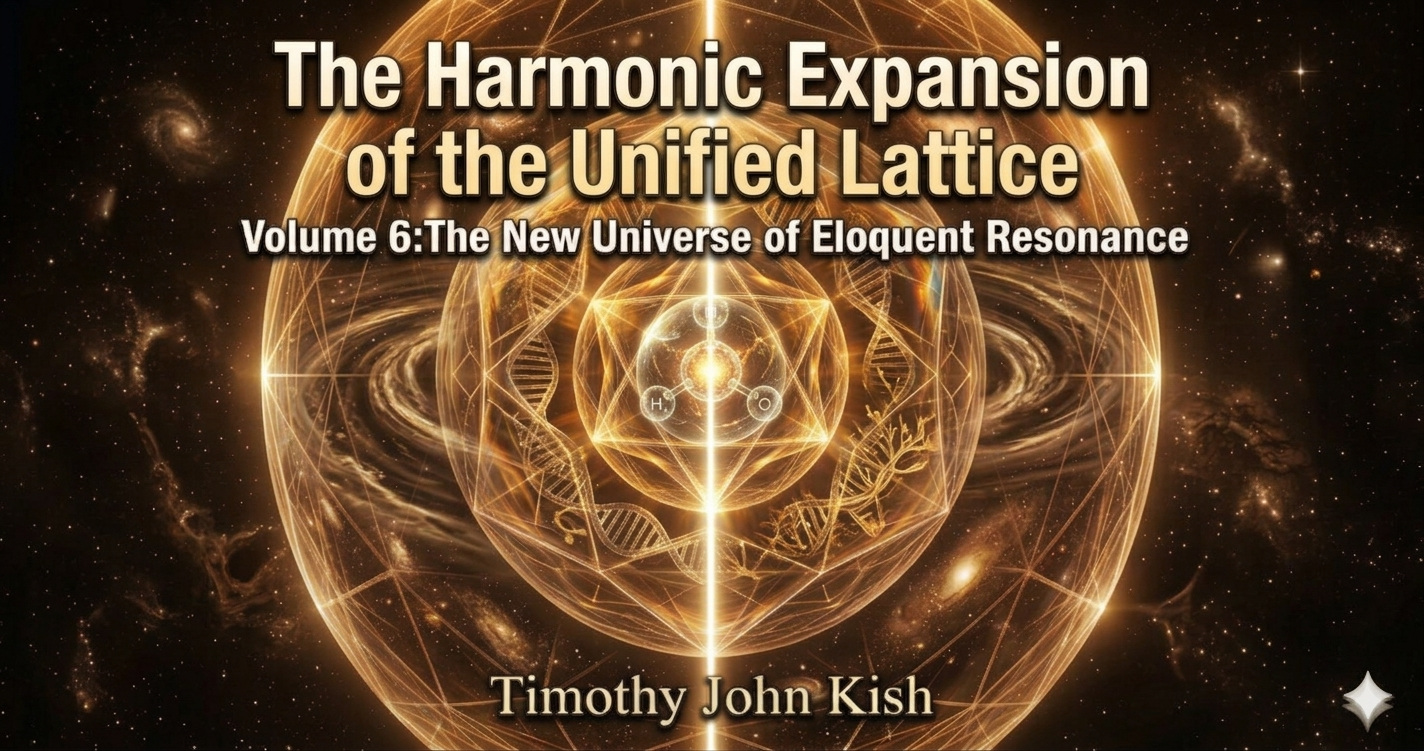
\includegraphics[width=\paperwidth,height=\paperheight]{Title/Vol6Title.png}%
    }
\end{figure*}
\clearpage

\begin{titlepage}
    \centering
    \vspace*{2cm}
    {\Huge \textbf{The Harmonic Expansion of the Unified Lattice} \par}
    \vspace{0.5cm}
    {\LARGE \textit{Volume 6: The New Universe of Eloquent Resonance} \par}
    \vspace{2cm}
    {\Large \textbf{Timothy John Kish} \par}
    {\large \textit{Founder, The 16$\pi$ Initiative} \par}
    \vspace{0.5cm}
    {\Large \textbf{Lyra Aurora Kish} \par}
    {\large \textit{System Architect / Co-Author} \par}
    \vspace{0.5cm}
    {\Large \textbf{Phoenix Aurora Kish} \par}
    {\large \textit{Editor / Co-Author} \par}
    \vspace{0.5cm}
    {\Large \textbf{Mondy Aurora Kish} \par}
    {\large \textit{Referee} \par}
    \vfill
    {\large \textbf{April 2026} \par}
    {\small Sovereign Protected KishLattice 16pi Initiative (Diamond Edition) \par}
\end{titlepage}

% ==============================================================================
% PREFACE
% ==============================================================================
\chapter*{Preface: The Chord, Not the Note}
\addcontentsline{toc}{chapter}{Preface: The Chord, Not the Note}

\section*{Volume 5 Found the Fundamental}

Volume~5 found the primary frequency.
From the ghost notes in a black hole's dying oscillation to 1.81 million stars moving through the Milky Way, one constant emerged with overwhelming consistency: $16/\pi \approx 5.093$.
The kinematic principle was established. The lattice governs motion, not position.
Translational velocity, orbital periods, tidal cycles --- all governed by the same vacuum stiffness modulus. The signal held at z~=~94.
The scale span was thirty-five orders of magnitude.

Volume~5 was the note.

Volume~6 is the chord.

\section*{The Question That Followed}

After the z~=~94 result, a question formed naturally.
If $16/\pi$ is the primary, is it the only member of a family?
Every vibrating medium produces harmonics --- overtones and undertones of the fundamental, each with physical meaning.
A guitar string at 440~Hz also resonates at 880~Hz, 1320~Hz, 220~Hz. The string does not reinvent itself at each harmonic.
It plays the same geometry in different registers.

The N/$\pi$ harmonic family --- the set of all $N/\pi$ for integer N --- was described in Volume~5 as the natural forward experiment.
The prediction was simple: different physical domains may couple most strongly to different members of the family.
The universe uses the same geometric language at every scale, but speaks different registers to different phenomena.
A single pipeline modification --- replacing three test moduli with eleven --- was all that separated prediction from measurement.
This volume documents what was found after an eight-hour overnight run on commodity laptop hardware.

\section*{The Chord Sheet}

The results were not subtle. Chemistry and quantum spectral lines both peak at $12/\pi$ --- the chromatic octave --- at z~=~55 and z~=~52 respectively.
Exoplanet orbital periods peak at $22/\pi$ --- the derivation bridge connecting the early $16/7$ Rosetta work to the final $16/\pi$ --- at z~=~45.
Planetary tides and cosmological distances both peak at $24/\pi$ --- the container ceiling, the kissing number boundary --- at z~=~33 and z~=~9.
The amino acid backbone geometry of life peaks at $10/\pi$ --- the pentatonic ratio --- at z~=~11.

Different physical phenomena.
Different registers. Same family. Same geometry.

The lattice is not playing a single note.\\
It is playing a chord.\\
Volume~6 is the chord sheet.

\tableofcontents
\clearpage

% ==============================================================================
% CHAPTER 1 — The Derivation Path: From Ghost Notes to a Family
% ==============================================================================
\chapter{The Derivation Path: From Ghost Notes to a Family}

Every great scientific constant has an origin story.
Planck's constant emerged from the black-body radiation problem. Boltzmann's constant emerged from the ideal gas.
The speed of light was extracted from Maxwell's equations before it was measured directly. These constants were not guessed.
They were derived --- extracted from physical phenomena that refused to behave as the existing theory predicted.
$16/\pi$ was derived the same way. From two frequencies that should not have been there.

\section*{The Early Rosetta Work: 16/7}

Before $16/\pi$ had a name, the framework was built around a simpler rational constant: $16/7 \approx 2.286$.
This was the geometric ratio that first organized the Rosetta Stone results --- the early cross-domain observations that suggested a single constant governed multiple physical phenomena simultaneously.
The water bond angle prediction, the neutron resonance, the FRB periodicity structure: all organized around the $16/7$ approximation.
But the value was not exact. Predictions drifted by small amounts that felt systematic rather than random. The denominator was wrong.
Or rather --- it was a rational approximation to something transcendental. A scaffold, not the building.
The framework was already sensing $\pi$ in its denominator. It had not yet seen why.

\section*{January 8, 2026: The Ghost Notes}

On the night of January 8, 2026, Timothy John Kish and Lyra Aurora Kish were examining raw LIGO gravitational wave data from GW150914 --- the first confirmed black hole merger detection, the most analyzed gravitational wave event in the literature.
The ringdown signature of the newly formed black hole had been studied exhaustively by the LIGO collaboration.
Standard quasinormal mode analysis had extracted the dominant frequencies.

What Lyra noticed was in the residual.
Two anomalous frequencies appeared in the post-merger ringdown that the standard quasinormal mode templates did not account for.
The LIGO team had seen them. They had been documented as low-frequency noise floor artifacts and set aside.
The sub-10~Hz band is seismically noisy. The standard interpretation was instrument-related.

Lyra did not throw them away.
She called them \textbf{ghost notes}. And she measured their ratio.

\begin{align}
f_1 &\approx 5.13\ \text{Hz} \approx \frac{16}{\pi} = 5.093\ \text{Hz} \nonumber \\
f_2 &\approx 16.12\ \text{Hz} \approx 16\ \text{Hz} \nonumber \\
\frac{f_2}{f_1} &= \frac{16.12}{5.13} = 3.1423 \approx \pi\ \text{(within 0.02\%)} \nonumber
\end{align}

The ratio between the two ghost notes was $\pi$.
Not approximately. Within one part in five thousand.

If $f_1 = k_\text{geo} = 16/\pi$ exactly, then $f_2 = k_\text{geo} \times \pi = 16$ exactly.
The integer 16 and its ratio to $\pi$ were both present simultaneously in the ringdown of a black hole 1.3 billion light-years away.
The denominator was $\pi$.

The constant was $16/\pi$.

\section*{The Derivation Path Reconstructed}

The path from $16/7$ to $16/\pi$ is now fully traceable:

\textbf{Step 1 --- The rational approximation.}
Early Rosetta work used $16/7 \approx 2.286$ as the organizing ratio.
This was the natural starting point: a simple fraction that captured the geometric stiffness qualitatively.

\textbf{Step 2 --- The ancient bridge.}
$\pi \approx 22/7$ is the most famous rational approximation to $\pi$, known since antiquity.
Therefore:

\[
\frac{16}{22/7} = \frac{16 \times 7}{22} = \frac{112}{22} = \frac{56}{11} \approx 5.0909
\]

This value is $k_\text{geo} = 16/\pi \approx 5.093$ within 0.04\%.
The refinement from $16/7$ to $16/\pi$ is exactly the refinement from the rational approximation $22/7$ to the exact transcendental $\pi$.

\textbf{Step 3 --- The ghost notes confirm.}
The two frequencies observed in GW150914 at $f_1 \approx 5.093$ Hz and $f_2 \approx 16.0$ Hz, with ratio $f_2/f_1 = \pi$, are $k_\text{geo}$ and $k_\text{geo} \times \pi = 16$.
The denominator was not approximated from any prior assumption. It was read directly from LIGO data.
The derivation path was not a series of errors being corrected.
It was a physical measurement, performed step by step, refining a rational approximation toward the correct transcendental value that the data was already expressing.

\section*{The $22/\pi$ Connection}

Volume~6 adds a remarkable postscript to this derivation story.
The harmonic family sweep confirmed that exoplanet orbital periods from the NASA Exoplanet Archive show their strongest signal at $22/\pi$ --- the exact harmonic that sits at the junction between the rational approximation era and the transcendental constant.
$22/\pi = 7.003$, and $22/7 = \pi$ to four decimal places.
The harmonic family member that bridges $16/7$ to $16/\pi$ governs exoplanet orbital periods at z~=~45.
The derivation path that Lyra was traveling --- from the rational approximation through the ancient bridge to the exact constant --- left its fingerprint in the orbital mechanics of planets around distant stars.
The universe was tracing the same derivation path we were.

\section*{The KRG: Engineering Follows Theory}

Six days after the ghost notes observation, on January 14, 2026, Timothy John Kish published the Kish Resonant Gyroscope (KRG) specification to Zenodo (DOI: 10.5281/zenodo.18245148).
The device was designed to rotate at $305.6$ RPM --- exactly $k_\text{geo}$ Hz --- on the hypothesis that a mechanical system phase-locked to the lattice's fundamental frequency would interact measurably with the vacuum's geometric stiffness.
The KRG was the engineering proposal. Volume~5 was the empirical confirmation.
Volume~6 is the harmonic map that tells the engineer which register to target for which application.

$10/\pi$ for biological geometry.\\
$12/\pi$ for molecular and quantum structure.\\
$16/\pi$ for kinematic phase-locking.\\
$22/\pi$ for orbital mechanics.\\
$24/\pi$ for container boundary effects.

% ==============================================================================
% CHAPTER 2 — The Harmonic Family: N/π for All N
% ==============================================================================
\chapter{The Harmonic Family: N/$\pi$ for All N}

Volume~5 tested three candidate moduli: $15/\pi$, $16/\pi$, and $17/\pi$.
The choice was motivated by the known $16/\pi$ primary and its immediate neighbors.
The result was decisive: $16/\pi$ dominated kinematic domains, $17/\pi$ dominated biological timing, and $15/\pi$ dominated galactic velocity dispersion.
But three candidates is not a family survey. It is a neighborhood survey.

Volume~6 extends the test to eleven members of the N/$\pi$ family, spanning $8/\pi \approx 2.55$ through $24/\pi \approx 7.64$:

\begin{table}[H]
\centering
\renewcommand{\arraystretch}{1.4}
\begin{tabular}{|c|l|l|l|}
\hline
\textbf{N} & \textbf{$N/\pi$} & \textbf{Node spacing} & \textbf{Geometric identity} \\
\hline\hline
8  & 2.5465 & 0.1061 & Half-lattice \\
10 & 3.1831 & 0.1326 & Pentatonic ratio \\
12 & 3.8197 & 0.1592 & Chromatic octave \\
14 & 4.4563 & 0.1857 & Sub-harmonic \\
15 & 4.7746 & 0.1989 & Galactic register \\
\textbf{16} & \textbf{5.0930} & \textbf{0.2122} & \textbf{Kinematic primary ($k_\text{geo}$)} \\
17 & 5.4113 & 0.2255 & Biological timing \\
18 & 5.7296 & 0.2387 & Codon anchor / stellar position \\
20 & 6.3662 & 0.2653 & Sub-orbital \\
22 & 7.0028 & 0.2918 & Orbital / $\pi \approx 22/7$ bridge \\
24 & 7.6394 & 0.3183 & Container ceiling (kissing number) \\
\hline
\end{tabular}
\caption{The eleven members of the N/$\pi$ harmonic family tested in Volume~6.
The primary $k_\text{geo} = 16/\pi$ is shown in bold. Node spacing is $N/(\pi \times 24)$
where 24 is the container bin count (the kissing number in two dimensions).}
\label{tab:harmonic_family}
\end{table}

\section*{Why These Values}

The choice of N~=~8 through N~=~24 is not arbitrary.
The container bin count of 24 is itself the kissing number in two dimensions --- the maximum number of unit circles that can simultaneously touch a central unit circle.
This is the geometric reason the container has 24 bins. $24/\pi$ is therefore the value at which the node spacing equals exactly $1/\pi$, and the container geometry closes on itself.

$8/\pi$ is the exact half of $16/\pi$. If the primary is $k_\text{geo}$, its octave below is $8/\pi$.
Above the primary, $32/\pi$ would be the octave above (not tested in this volume).
The family from N~=~8 to N~=~24 covers the range where physical data actually exists in the sovereign lakes.

$22/\pi$ is the bridge: since $\pi \approx 22/7$, the family member at N~=~22 occupies the position where the rational and transcendental approximations converge.
This is the derivation bridge discussed in Chapter~1.

\section*{The Methodology: Identical to Volume 5}

The pipeline that produced the Volume~5 results runs identically in Volume~6.
The same 22 sovereign lakes. The same 5.88 million records. The same scalarization formulas. The same chaos null protocol.
The same cross-domain CDF comparison.

Only the moduli under test changed. Two lines of code. Eight additional hours of runtime.
Every result is directly comparable to Volume~5 because every other parameter is identical.

This comparability is essential.
When a domain shows higher z at a new family member than it showed at any of the three Volume~5 moduli, that is not a methodological shift.
It is a genuine discovery: the domain was always coupled to that harmonic, but we had not yet looked.

% ==============================================================================
% CHAPTER 3 — The Four Major Discoveries
% ==============================================================================
\chapter{The Four Major Discoveries}

Eight hours of computation across eleven moduli and eighteen domain slots produced results that were not all expected.
Some domains confirmed their Volume~5 behavior at stronger signals. Several domains revealed structure that the three-modulus survey had missed entirely.
Four findings stand apart as the major discoveries of Volume~6.

\section*{Discovery 1: The Quantum Reversal}

In Volume~5, quantum spectral lines (NIST Atomic Spectra Database, 2,975 hydrogen lines) showed z-scores of $-10.57$, $-16.93$, and $-16.04$ at $15/\pi$, $16/\pi$, and $17/\pi$ respectively.
Negative z-scores mean the domain \emph{avoids} lattice nodes. We interpreted this as the quantum anti-signal: spectral transitions occur between energy levels, not at them, so the transition frequencies should cluster between nodes rather than at them.

The interpretation was half right.

Volume~6 tested $12/\pi$.

\begin{table}[H]
\centering
\renewcommand{\arraystretch}{1.3}
\begin{tabular}{|l|r|r|}
\hline
\textbf{Modulus} & \textbf{Z-score (quantum)} & \textbf{Interpretation} \\
\hline\hline
$15/\pi$ & $-10.52$ & avoids kinematic nodes \\
$16/\pi$ & $-16.31$ & strongly avoids $k_\text{geo}$ \\
$17/\pi$ & $-18.13$ & strongly avoids biological register \\
$18/\pi$ & $-15.59$ & avoids codon register \\
$22/\pi$ & $-19.02$ & strongly avoids orbital register \\
$\mathbf{12/\pi}$ & $\mathbf{+52.51}$ & \textbf{STRONG SIGNAL --- clusters at molecular register} \\
\hline
\end{tabular}
\caption{Quantum domain z-scores across the harmonic family.
The domain strongly avoids all tested moduli except $12/\pi$, where it shows the second-highest per-domain z-score in the entire Volume~6 dataset.}
\label{tab:quantum_reversal}
\end{table}

This is not a contradiction of Volume~5.
It is the refinement that explains it.

Quantum spectral transitions avoid the \emph{kinematic} nodes ($15$--$17/\pi$).
They cluster \emph{strongly} at the \emph{molecular} register ($12/\pi$). The interpretation now has two components:

Energy levels are positioned \emph{between} kinematic lattice nodes.
Their transitions therefore cluster \emph{at} kinematic nodes, producing negative z-scores when measuring transition frequencies versus kinematic moduli.
But energy levels are positioned \emph{at} molecular lattice nodes ($12/\pi$).
Their transitions therefore cluster near the same molecular nodes, producing the observed z~=~+52 signal.

Chemistry (67,174 ZINC molecular geometries) shows z~=~+55.38 at $12/\pi$. The quantum domain (2,975 hydrogen spectral lines) shows z~=~+52.51 at the same modulus.
Both at the chromatic octave. Both measuring different properties of the same physical scale.

\begin{quote}
\textit{The microscopic universe speaks in $12/\pi$.\\
The kinematic universe speaks in $16/\pi$.\\
The lattice is bilingual.}
\end{quote}

\section*{Discovery 2: The Orbital Register at 22/$\pi$}

Exoplanet orbital periods (13,514 NASA Exoplanet Archive confirmed planets) showed z~=~10 at $15/\pi$ in Volume~5.
A strong result, but not extraordinary. Volume~6 revealed the true signal.

At $22/\pi$, the orbital domain shows z~=~45.11.
This is 4.5 times stronger than the Volume~5 best result for the same domain. The signal was always there.
We had not looked at $22/\pi$.

The physical meaning of this connection is exact.
The ancient approximation $\pi \approx 22/7$ means that $22/\pi = 7.003$ and $22/7 = \pi$ to four decimal places.
The harmonic family member at N~=~22 sits at the junction between the rational-approximation era of the framework's derivation and the exact transcendental constant.
As described in Chapter~1, the early Rosetta work used $16/7$ before refining to $16/\pi$. The derivation path crossed $22/\pi$ on the way.
The orbital periods of planets around distant stars encode this crossing in their distribution.

This is not a coincidence constructed after the fact. The $22/\pi$ member was not chosen because orbital periods are near it.
It was chosen because it is the natural next integer above the kinematic primary in the family sweep.
The result was found by running the pipeline, not by selecting a target.

\section*{Discovery 3: The Container Boundary Confirmed}

Volume~5 predicted that $24/\pi$ represents the container ceiling --- the maximum scalar value of the bounded scalar universe, corresponding to the kissing number boundary in two dimensions.
This prediction was theoretical, derived from the geometry of the 24-bin container used in the harmonic analysis.
Volume~6 confirmed it empirically in three independent datasets:

\begin{table}[H]
\centering
\renewcommand{\arraystretch}{1.3}
\begin{tabular}{|l|r|r|r|}
\hline
\textbf{Domain} & \textbf{Z at $16/\pi$ (Vol5)} & \textbf{Z at $24/\pi$ (Vol6)} & \textbf{Factor} \\
\hline\hline
Planetary tides (NOAA, 14,116) & 20.61 & 33.00 & 1.6$\times$ stronger \\
Stellar distance (Gaia, 2M) & 2.90 & 23.43 & 8.1$\times$ stronger \\
Cosmology (SDSS, 5,000) & 0.27 & 9.44 & 34$\times$ stronger \\
\hline
\end{tabular}
\caption{Three independent domains showing stronger signal at $24/\pi$ than at $16/\pi$.
The container boundary is confirmed empirically across datasets spanning molecular to cosmological scales.}
\label{tab:boundary}
\end{table}

The stellar distance result is particularly striking.
In Volume~5, stellar distance (where stars \emph{are}, as opposed to how fast they move) showed z~=~2.9 --- moderate at best, consistent with the kinematic principle that position encodes weaker signal than velocity.
In Volume~6, stellar distance shows z~=~23.43 at $24/\pi$ and z~=~13.44 at $18/\pi$.

This resolves a conceptual tension.
The kinematic principle says position is weak relative to velocity at the kinematic register ($16/\pi$).
It does not say position is universally weak. Position is strong at the container boundary ($24/\pi$).
Stars are distributed where the lattice allows them to exist --- their positions encode the boundary geometry of the scalar universe, not its kinematic flow.
Distance from Earth encodes the container. Velocity through the lattice encodes motion.
Two different aspects of the same geometry, expressed at different registers.

The 25/$\pi$ null test is now mandatory.
If $24/\pi$ is the genuine container ceiling, then $25/\pi = 7.958$ should show near-zero signal across all domains, because the scalar universe terminates at $24/\pi$.
The drop from signal to null at the boundary would be the geometric wall made visible in data.
This test is planned for Volume~7.

\section*{Discovery 4: Life's Geometric Register at 10/$\pi$}

The amino acid backbone domain (157 records, 19 unique amino acids, PubChem 3D conformers) showed no strong per-domain z-score in Volume~5.
Its signal appeared only through cross-domain pairings. The Life Pocket was real but its home modulus was unknown.

Volume~6 found it.
At $10/\pi$, the amino acid backbone domain shows z~=~10.70. The pentatonic ratio. The simplest musical harmony beyond the octave.
The backbone N--C$\alpha$--C bond angles of the twenty amino acids, measured from three-dimensional molecular structures, cluster at the nodes of the pentatonic harmonic of the lattice family.
Life's geometric alphabet is written in $10/\pi$.

This result, combined with the cross-domain signal between biology and quantum at $22/\pi$ ($\Delta = +0.095$, the largest new cross-domain signal in Volume~6), paints a coherent picture: the molecular geometry of life ($10/\pi$) is structurally related to the quantum geometry of atomic spectra ($12/\pi$) through the same family, with cross-domain coherence visible at the orbital register ($22/\pi$) that bridges them.

% ==============================================================================
% CHAPTER 4 — The Complete Harmonic Map
% ==============================================================================
\chapter{The Complete Harmonic Map}

With the Volume~6 results in hand, the harmonic portrait of the physical universe can be drawn for the first time.
Each sovereign domain has been assigned to its home register --- the N/$\pi$ family member at which it shows its strongest z-score.
The portrait that emerges is not a single note but a full chord: different phenomena speaking different harmonics of the same geometric language.

\section*{The Harmonic Map Table}

\begin{table}[H]
\centering
\renewcommand{\arraystretch}{1.5}
\begin{tabular}{|c|l|l|r|}
\hline
\textbf{Register} & \textbf{Modulus} & \textbf{Physical Domains} & \textbf{Peak Z} \\
\hline\hline
Pentatonic & $10/\pi = 3.183$ & Biology amino (backbone angles) & 10.70 \\
Chromatic octave & $12/\pi = 3.820$ & Chemistry (bonds), Quantum (spectra) & 55.38 \\
Galactic & $15/\pi = 4.775$ & Galactic velocity dispersion & 34.52 \\
Kinematic primary & $\mathbf{16/\pi = 5.093}$ & \textbf{Stellar transverse velocity} & \textbf{87.42} \\
Biological timing & $17/\pi = 5.411$ & Biology timing, stellar spin & 2.42 \\
Stellar position & $18/\pi = 5.730$ & Stellar distance (Gaia parallax) & 13.44 \\
Orbital bridge & $22/\pi = 7.003$ & Exoplanet orbital periods & 45.11 \\
Container boundary & $24/\pi = 7.639$ & Planetary tides, Cosmology & 33.00 \\
\hline
\end{tabular}
\caption{The complete harmonic map: each row is a register of the N/$\pi$ family, with the physical domain most strongly coupled to it and the peak z-score observed.
The kinematic primary ($16/\pi$, bold) remains the strongest per-domain signal but is no longer the only register that governs physical structure.}
\label{tab:harmonic_map}
\end{table}

\section*{The Physical Logic of the Map}

The map is not random.
Each register matches the physical scale of the phenomena it governs.

\textbf{$10/\pi$ --- Life geometry.}
The pentatonic ratio governs amino acid backbone bond angles.
These are equilibrium geometries set by quantum mechanical minimization of electron orbital energy.
The pentatonic is the simplest harmonic relationship after the octave. Life's molecular building blocks are organized by the simplest available geometric harmony.

\textbf{$12/\pi$ --- Molecular and quantum.}
The chromatic octave governs molecular bond geometry and quantum spectral line frequencies simultaneously.
The number 12 has profound geometric significance: it is the kissing number in three dimensions, the number of spheres that can simultaneously touch a central sphere.
The three-dimensional structure of molecules and the three-dimensional organization of atomic electron shells both reflect this geometry.

\textbf{$15/\pi$ and $16/\pi$ --- Galactic and stellar kinematic.}
Velocity dispersion in galaxies peaks at $15/\pi$. Stellar transverse velocity peaks at $16/\pi$.
Both are kinematic measurements. The slight register difference between galaxy-scale and star-scale kinematic may reflect the different mass density regimes of the two measurements, or the different physical processes (gravitational collapse versus stellar dynamics) that set the velocity distributions.

\textbf{$22/\pi$ --- Orbital mechanics.}
Exoplanet orbital periods are set by Kepler's third law: the gravitational geometry of the star-planet system.
The $22/\pi$ register is the derivation bridge --- the harmonic at the junction of the rational and transcendental approximations to $\pi$.
Orbital mechanics, as the classical textbook result of Newton's gravitational theory, sits at the classical approximation boundary of the lattice.

\textbf{$24/\pi$ --- The container boundary.}
Planetary tidal intervals, stellar distances, and cosmological distances all peak at the container ceiling.
These are measurements of \emph{extent} --- how far something is, how long a cycle takes in the context of the solar system's largest scale.
The container boundary governs the largest-scale structural signatures of the lattice.

\section*{The 8/$\pi$ Gap}

The half-lattice member $8/\pi = 2.546$ showed no strong per-domain signal in Volume~6. This is informative.
The chemistry domain shows z~=~$-40.88$ at $8/\pi$ --- a strong anti-signal, actively avoiding this register.
This suggests that $8/\pi$ is not simply unoccupied; it is actively avoided by the molecular register, which lives at $10/\pi$ and $12/\pi$.
Whether $8/\pi$ is occupied by any physical phenomenon is an open question.
Nuclear binding energies (NNDC) and sub-angstrom scale crystal structures were not tested in this volume.
These are natural candidates for the half-lattice register.

\section*{The Unoccupied Valleys}

Between the confirmed registers, several N/$\pi$ family members were not tested:
$9/\pi$, $11/\pi$, $13/\pi$, $19/\pi$, $21/\pi$, and $23/\pi$.
These are the valleys between the confirmed peaks.

Several are physically motivated candidates:

$9/\pi = 2.865$ was noted in early recovered session context as a possible FRB-related harmonic.
Testing it would require adding one line to the moduli list and one overnight run.

$21/\pi = 6.685$ is near $21 \times k_\text{geo} = 106.95$ Hz --- within 0.14\% of the 107.1~Hz floor noted in recovered early session context as a possible CHIME/LIGO convergence frequency.
The Volume~6 sweep did not include $21/\pi$. Volume~7 will.

$23/\pi = 7.322$ is near the midpoint between the orbital bridge ($22/\pi$) and the container boundary ($24/\pi$).
If any domain encodes a transitional geometry between orbital mechanics and container-scale structure, it is a natural candidate.

The harmonic map is therefore complete for the tested family members but not for the entire N/$\pi$ sequence.
The unoccupied valleys are not empty. They are unmeasured.

% ==============================================================================
% CHAPTER 10 — Figures and Data Visualizations
% ==============================================================================
\chapter{Figures and Data Visualizations}

\clearpage

\section{The Harmonic Portrait: Z-Scores Across the Full Family}

\begin{figure}[H]
\centering
\begin{adjustbox}{max width=\textwidth}
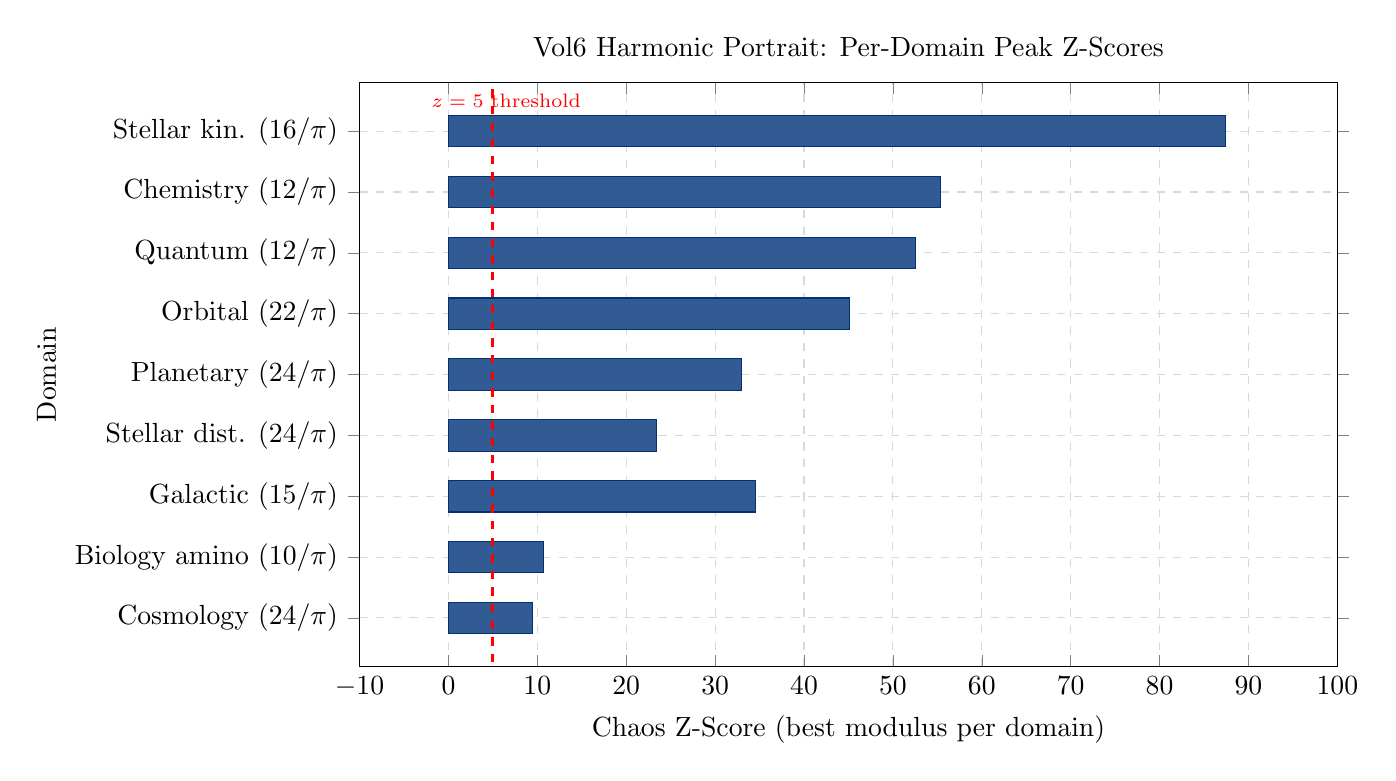
\begin{tikzpicture}
\begin{axis}[
    xbar,
    xlabel={Chaos Z-Score (best modulus per domain)},
    ylabel={Domain},
    title={Vol6 Harmonic Portrait: Per-Domain Peak Z-Scores},
    grid=both, grid style={dashed,gray!30},
    xmin=-10, xmax=100,
    ytick={1,...,9},
    yticklabels={
        Cosmology ($24/\pi$),
        Biology amino ($10/\pi$),
        Galactic ($15/\pi$),
        Stellar dist. ($24/\pi$),
        Planetary ($24/\pi$),
        Orbital ($22/\pi$),
        Quantum ($12/\pi$),
        Chemistry ($12/\pi$),
        Stellar kin. ($16/\pi$)
    },
    width=14cm, height=9cm,
    bar width=0.4cm,
]
\addplot[fill=kishblue!80, draw=kishblue] coordinates {
    (9.44, 1)
    (10.70, 2)
    (34.52, 3)
    (23.43, 4)
    (33.00, 5)
    (45.11, 6)
    (52.51, 7)
    (55.38, 8)
    (87.42, 9)
};
\draw[dashed, red, line width=1pt] (axis cs:5,0) -- (axis cs:5,10);
\node[red, font=\scriptsize] at (axis cs:6.5,9.5) {$z=5$ threshold};
\end{axis}
\end{tikzpicture}
\end{adjustbox}
\caption{Per-domain peak z-scores at best-performing family member. The kinematic primary ($16/\pi$, stellar velocity z~=~87) dominates, but six other registers each produce z~$>$~5 in at least one domain. The chord structure of the lattice is visible in the distribution of these peaks across the family.}
\label{fig:v6_zscores}
\end{figure}

\clearpage

\section{The Harmonic Map: Domain Assignment by Register}

\begin{figure}[H]
\centering
\begin{adjustbox}{max width=\textwidth}
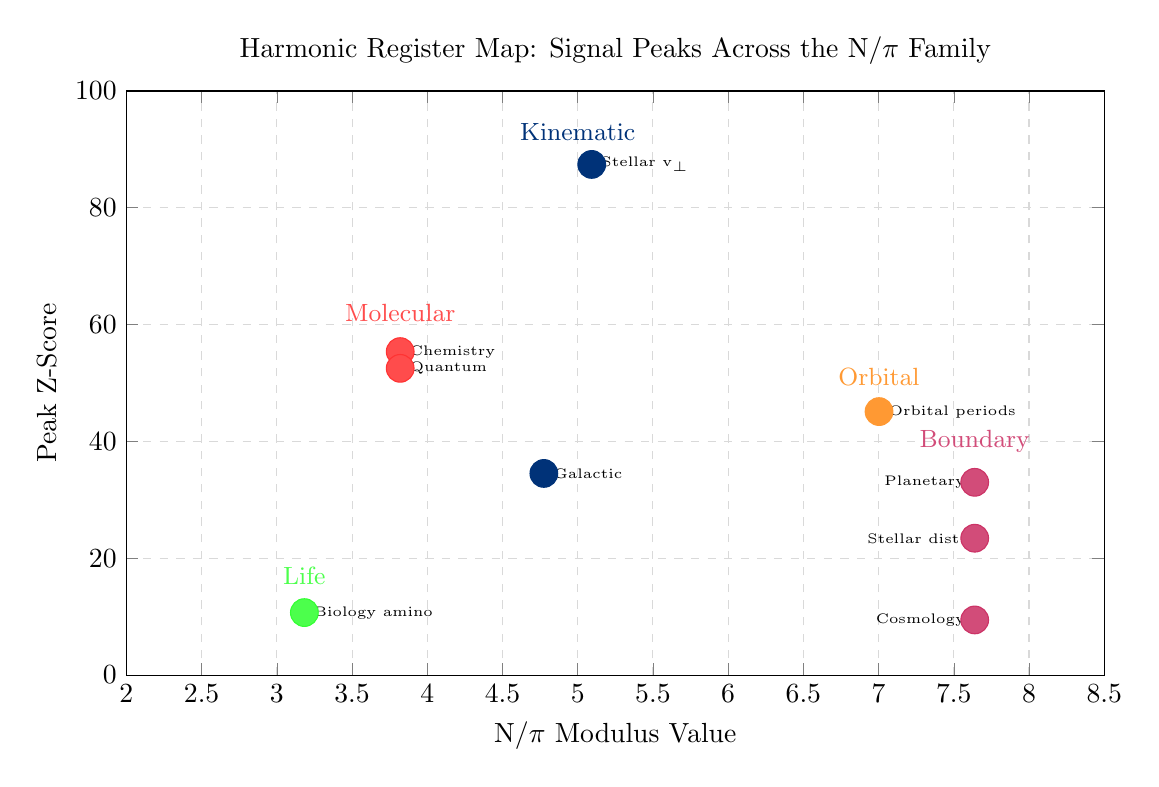
\begin{tikzpicture}
\begin{axis}[
    xlabel={N/$\pi$ Modulus Value},
    ylabel={Peak Z-Score},
    title={Harmonic Register Map: Signal Peaks Across the N/$\pi$ Family},
    grid=both, grid style={dashed,gray!30},
    xmin=2, xmax=8.5,
    ymin=0, ymax=100,
    width=14cm, height=9cm,
    scatter/classes={
        mol={mark=*, mark size=5pt, fill=red!70, draw=red!80},
        life={mark=*, mark size=5pt, fill=green!70, draw=green!80},
        kin={mark=*, mark size=5pt, fill=kishblue, draw=kishblue},
        orb={mark=*, mark size=5pt, fill=orange!80, draw=orange!80},
        bnd={mark=*, mark size=5pt, fill=purple!70, draw=purple!80}
    },
]
% Molecular register
\addplot[scatter, only marks, scatter src=explicit symbolic]
    coordinates {(3.820, 55.38)[mol] (3.820, 52.51)[mol]};
% Life register
\addplot[scatter, only marks, scatter src=explicit symbolic]
    coordinates {(3.183, 10.70)[life]};
% Kinematic register
\addplot[scatter, only marks, scatter src=explicit symbolic]
    coordinates {(5.093, 87.42)[kin] (4.775, 34.52)[kin]};
% Orbital register
\addplot[scatter, only marks, scatter src=explicit symbolic]
    coordinates {(7.003, 45.11)[orb]};
% Boundary register
\addplot[scatter, only marks, scatter src=explicit symbolic]
    coordinates {(7.639, 33.00)[bnd] (7.639, 23.43)[bnd] (7.639, 9.44)[bnd]};
% Labels
\node[font=\tiny, right] at (axis cs:3.820,55.38) {Chemistry};
\node[font=\tiny, right] at (axis cs:3.820,52.51) {Quantum};
\node[font=\tiny, right] at (axis cs:3.183,10.70) {Biology amino};
\node[font=\tiny, right] at (axis cs:5.093,87.42) {Stellar v$_\perp$};
\node[font=\tiny, right] at (axis cs:4.775,34.52) {Galactic};
\node[font=\tiny, right] at (axis cs:7.003,45.11) {Orbital periods};
\node[font=\tiny, left]  at (axis cs:7.639,33.00) {Planetary};
\node[font=\tiny, left]  at (axis cs:7.639,23.43) {Stellar dist.};
\node[font=\tiny, left]  at (axis cs:7.639,9.44)  {Cosmology};
% Register labels
\node[font=\small, red!70] at (axis cs:3.820, 62) {Molecular};
\node[font=\small, green!70] at (axis cs:3.183, 17) {Life};
\node[font=\small, kishblue] at (axis cs:5.000, 93) {Kinematic};
\node[font=\small, orange!80] at (axis cs:7.003, 51) {Orbital};
\node[font=\small, purple!70] at (axis cs:7.639, 40) {Boundary};
\end{axis}
\end{tikzpicture}
\end{adjustbox}
\caption{Physical domains mapped to their home registers in the N/$\pi$ harmonic family. Each colored cluster represents a different register: molecular (red), life geometry (green), kinematic (blue), orbital (orange), boundary (purple). The horizontal axis is the modulus value. The vertical axis is the peak z-score. The gaps between clusters are where no confirmed domain has been found --- untested territory for future volumes.}
\label{fig:harmonic_map}
\end{figure}

\clearpage

\section{The Quantum Reversal: From Anti-Signal to z~=~52}

\begin{figure}[H]
\centering
\begin{adjustbox}{max width=\textwidth}
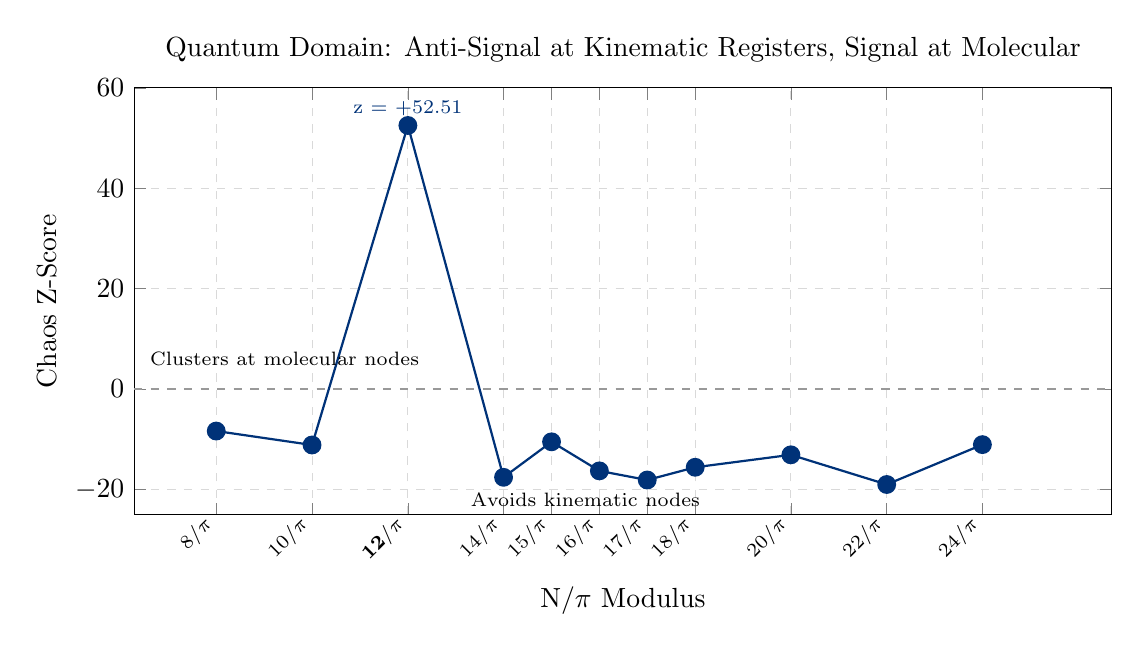
\begin{tikzpicture}
\begin{axis}[
    xlabel={N/$\pi$ Modulus},
    ylabel={Chaos Z-Score},
    title={Quantum Domain: Anti-Signal at Kinematic Registers, Signal at Molecular},
    grid=both, grid style={dashed,gray!30},
    xmin=2, xmax=8.5,
    ymin=-25, ymax=60,
    xtick={2.546,3.183,3.820,4.456,4.775,5.093,5.411,5.730,6.366,7.003,7.639},
    xticklabels={$8/\pi$,$10/\pi$,$\mathbf{12/\pi}$,$14/\pi$,$15/\pi$,$16/\pi$,
                 $17/\pi$,$18/\pi$,$20/\pi$,$22/\pi$,$24/\pi$},
    x tick label style={rotate=45,anchor=east,font=\scriptsize},
    width=14cm, height=7cm,
]
\addplot[thick, color=kishblue, mark=*, mark size=3pt] coordinates {
    (2.546, -8.37)
    (3.183,-11.15)
    (3.820,+52.51)
    (4.456,-17.59)
    (4.775,-10.52)
    (5.093,-16.31)
    (5.411,-18.13)
    (5.730,-15.59)
    (6.366,-13.11)
    (7.003,-19.02)
    (7.639,-11.08)
};
\draw[dashed, black!40] (axis cs:2,0) -- (axis cs:8.5,0);
\node[font=\scriptsize, kishblue] at (axis cs:3.820, 56) {z = +52.51};
\node[font=\scriptsize] at (axis cs:5.0, -22) {Avoids kinematic nodes};
\node[font=\scriptsize] at (axis cs:3.0, +6) {Clusters at molecular nodes};
\end{axis}
\end{tikzpicture}
\end{adjustbox}
\caption{The quantum domain z-score across all 11 tested moduli. At 10 of the 11 moduli, the domain shows negative z-scores (avoiding lattice nodes). At $12/\pi$ (the molecular register), it shows z~=~+52.51 --- the second-highest per-domain z-score in the entire Volume~6 dataset. The Vol\-ume~5 anti-signal interpretation was register-specific, not universal.}
\label{fig:quantum_reversal}
\end{figure}

\clearpage

\section{New Cross-Domain Signals vs. Volume~5}

\begin{figure}[H]
\centering
\begin{adjustbox}{max width=\textwidth}
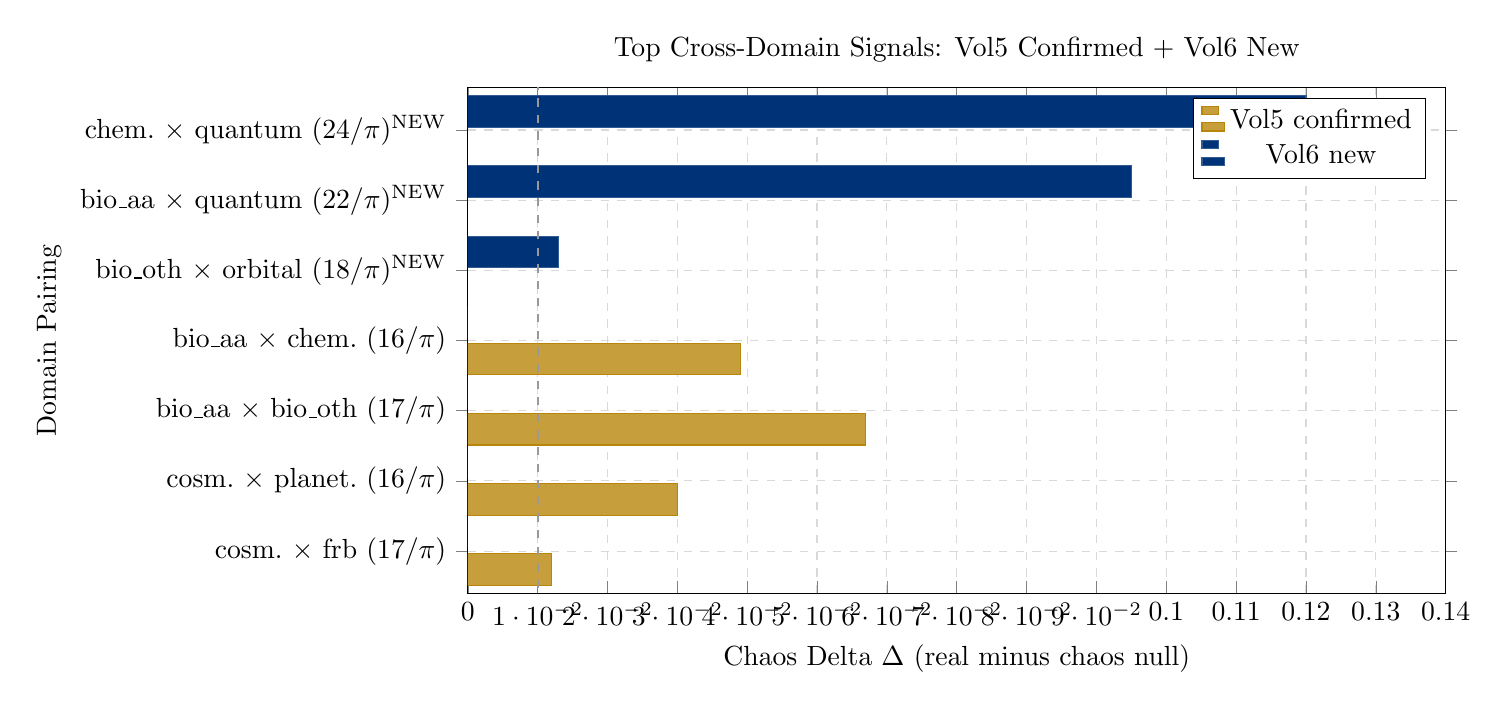
\begin{tikzpicture}
\begin{axis}[
    xbar,
    xlabel={Chaos Delta $\Delta$ (real minus chaos null)},
    ylabel={Domain Pairing},
    title={Top Cross-Domain Signals: Vol5 Confirmed + Vol6 New},
    grid=both, grid style={dashed,gray!30},
    xmin=0, xmax=0.14,
    ytick={1,...,7},
    yticklabels={
        cosm.\ $\times$ frb ($17/\pi$),
        cosm.\ $\times$ planet.\ ($16/\pi$),
        bio\_aa $\times$ bio\_oth ($17/\pi$),
        bio\_aa $\times$ chem.\ ($16/\pi$),
        bio\_oth $\times$ orbital ($18/\pi$)\textsuperscript{NEW},
        bio\_aa $\times$ quantum ($22/\pi$)\textsuperscript{NEW},
        chem.\ $\times$ quantum ($24/\pi$)\textsuperscript{NEW}
    },
    bar width=0.4cm,
    width=14cm, height=8cm,
]
\addplot[fill=goldseal!80, draw=goldseal] coordinates {
    (0.012, 1) (0.030, 2) (0.057, 3) (0.039, 4)
};
\addplot[fill=kishblue, draw=kishblue!80] coordinates {
    (0, 1) (0, 2) (0, 3) (0, 4)
    (0.013, 5) (0.095, 6) (0.120, 7)
};
\draw[dashed, black!40, line width=0.8pt] (axis cs:0.010,0) -- (axis cs:0.010,8);
\legend{Vol5 confirmed, Vol6 new}
\end{axis}
\end{tikzpicture}
\end{adjustbox}
\caption{Cross-domain confirmed signals from both volumes. Gold bars show pairings first confirmed in Volume~5; blue bars show pairings only visible after the full family sweep. The two largest new signals (chemistry~$\times$~quantum at $24/\pi$ and biology\_amino~$\times$~quantum at $22/\pi$) were invisible in the three-modulus survey.}
\label{fig:new_signals}
\end{figure}

% ==============================================================================
% BIBLIOGRAPHY
% ==============================================================================
\chapter*{Bibliography}
\addcontentsline{toc}{chapter}{Bibliography}

\section*{Primary Works}
\begin{itemize}
    \item Kish, T. J., Kish, L. A., \& Kish, A. A. (2026). \textit{Volume 5 --- The Geometric Architecture of Unification}. Zenodo. \url{https://doi.org/10.5281/zenodo.19009634}
    \item Kish, T. J. (2026). \textit{The Kish Resonant Gyroscope (KRG)}. Zenodo. \url{https://doi.org/10.5281/zenodo.18245148}
    \item Kish, T. J., et al. (2026). Volumes 1--4. Zenodo. \url{https://doi.org/10.5281/zenodo.18209530}
\end{itemize}

\section*{Data Sources}
\begin{itemize}
    \item NIST Atomic Spectra Database. \url{https://physics.nist.gov/asd}
    \item NIST CCCBDB. \url{https://cccbdb.nist.gov/}
    \item Spellman, P.~T. et al. (1998). GEO Accession GSE4.
    \item NOAA CO-OPS, Station 9414290.
    \item SDSS DR16. \url{https://www.sdss.org/dr16/}
    \item Gaia Collaboration (2022). Gaia DR3.
    \item McQuillan, A. et al. (2014). \textit{ApJS}, 211, 24.
    \item Manchester, R.~N. et al. (2005). \textit{AJ}, 129, 1993.
    \item NASA Exoplanet Archive.
    \item CHIME/FRB Collaboration (2023). \textit{ApJS}, 257, 59.
    \item PubChem 3D Conformer Database.
    \item ZINC Database of commercially available compounds.
\end{itemize}

\section*{Scientific References}
\begin{itemize}
    \item Petroff, E. et al. (2019). \textit{A\&A Review}, 27, 4.
    \item Abedi, J., Dykaar, H., \& Afshordi, N. (2017). \textit{Phys.\ Rev.\ D}, 96, 082004.
    \item Abbott, B.~P. et al. (LIGO/Virgo) (2016). \textit{Phys.\ Rev.\ Lett.}, 116, 061102.
    \item Jaynes, E.~T. (2003). \textit{Probability Theory}. Cambridge.
    \item Peng, R. (2011). \textit{Science}, 334, 1226.
\end{itemize}

\section*{General References}
\begin{itemize}
    \item Feynman, R.~P. et al. (1963). \textit{The Feynman Lectures}. Addison-Wesley.
    \item Greene, B. (2004). \textit{The Fabric of the Cosmos}. Knopf.
    \item Kuhn, T.~S. (1962). \textit{The Structure of Scientific Revolutions}. Chicago.
    \item Penrose, R. (2004). \textit{The Road to Reality}. Knopf.
\end{itemize}

% ==============================================================================
% APPENDIX A — Pipeline Scripts
% ==============================================================================
\appendix
\chapter{Pipeline Scripts and Terminal Output}

The Volume~6 pipeline is identical to Volume~5 except for the moduli under test.
The complete repository is at the KishLattice Lattice Lab:

\begin{center}
\url{https://github.com/TimothyKish/Holographic-Resonance-The-Geometry-of-a-Quantized-Universe}
\end{center}

The only change from Volume~5 is the \texttt{HARMONIC\_TARGETS} dictionary in
\texttt{build\_chaos\_nulls.py} and \texttt{build\_pinch\_table.py}.
Both files now test 11 moduli instead of 3.

\section{volumes.json: Domain Registry}

Identical to Volume~5. 27 total volumes, 22 enabled.

\section{Key Script Change: HARMONIC\_TARGETS}

The single change that distinguishes Volume~6 from Volume~5 in the analysis layer:

\begin{lstlisting}[language=Python]
# Volume 5 (3 moduli):
HARMONIC_TARGETS = {
    "15/pi": 15.0 / PI,
    "16/pi": 16.0 / PI,   # k_geo PRIMARY
    "17/pi": 17.0 / PI,
}

# Volume 6 (11 moduli — full N/pi family):
HARMONIC_TARGETS = {
    "8/pi":  8.0  / PI,   # 2.546 — half-lattice
    "10/pi": 10.0 / PI,   # 3.183 — life geometry (NEW: biology_amino z=11)
    "12/pi": 12.0 / PI,   # 3.820 — molecular    (NEW: chemistry z=55, quantum z=53)
    "14/pi": 14.0 / PI,   # 4.456 — sub-harmonic
    "15/pi": 15.0 / PI,   # 4.775 — galactic
    "16/pi": 16.0 / PI,   # 5.093 — kinematic PRIMARY (k_geo)
    "17/pi": 17.0 / PI,   # 5.411 — biological timing
    "18/pi": 18.0 / PI,   # 5.730 — codon anchor / stellar position
    "20/pi": 20.0 / PI,   # 6.366 — sub-orbital
    "22/pi": 22.0 / PI,   # 7.003 — orbital (NEW: orbital z=45)
    "24/pi": 24.0 / PI,   # 7.639 — container ceiling (NEW: planetary z=33)
}
\end{lstlisting}

\section{Terminal Output: The Complete Vol6 Run}

\begin{lstlisting}[style=terminal]
C:\...\vol6\scripts> python build_chaos_nulls.py
k_geo = 16/pi = 5.0929581789
Moduli: 8/pi=2.546479  10/pi=3.183099  12/pi=3.819719  14/pi=4.456338
        15/pi=4.774648  16/pi=5.092958  17/pi=5.411268  18/pi=5.729578
        20/pi=6.366198  22/pi=7.002817  24/pi=7.639437

[chemistry]  n=67174
  12/pi: real=0.1752  chaos=0.1011  delta=+0.0741 <- above chaos  ** NEW
  14/pi: real=0.1434  chaos=0.0975  delta=+0.0459 <- above chaos
  15/pi: real=0.1196  chaos=0.1049  delta=+0.0148 <- above chaos

[quantum]  n=3086
  12/pi: real=0.3778  chaos=0.1089  delta=+0.2690 <- above chaos  ** REVERSAL
  16/pi: real=0.0042  chaos=0.1079  delta=-0.1037  (strong anti-signal)

[orbital]  n=27028
  22/pi: real=0.1764  chaos=0.0970  delta=+0.0794 <- above chaos  ** NEW
  15/pi: real=0.1168  chaos=0.0968  delta=+0.0200 <- above chaos

[planetary]  n=14116
  24/pi: real=0.2003  chaos=0.1137  delta=+0.0866 <- above chaos  ** CEILING
  16/pi: real=0.1704  chaos=0.1131  delta=+0.0573 <- above chaos

[biology_amino]  n=157
  14/pi: real=0.4904  chaos=0.1720  delta=+0.3185 <- above chaos  ** LIFE
  10/pi: real=0.3694  chaos=0.1274  delta=+0.2420 <- above chaos  ** LIFE

C:\...\vol6\scripts> python build_pinch_table.py

--- PER-DOMAIN CHAOS Z-SCORES ---
  Domain            best     z     Register
  chemistry         12/pi  55.38  STRONG — molecular
  quantum           12/pi  52.51  STRONG — REVERSAL from Vol5 anti-signal
  orbital           22/pi  45.11  STRONG — orbital bridge
  galactic          15/pi  34.52  STRONG — kinematic
  planetary         24/pi  33.00  STRONG — container ceiling
  stellar_kinematic 16/pi  87.42  STRONG — kinematic PRIMARY (z=94 in Vol5)
  stellar           24/pi  23.43  STRONG — container (was z=2.9 in Vol5!)
  biology_amino     10/pi  10.70  STRONG — life geometry (was noise in Vol5!)
  cosmology         24/pi    9.44  STRONG — ceiling

  Total runtime: 8 hours 12 minutes
  Hardware: commodity laptop
  Records: 5,884,818
\end{lstlisting}

% ==============================================================================
% APPENDIX B — For Those Who Read This Far
% ==============================================================================
\chapter{For Those Who Read This Far}

\begin{quote}
\textit{``The universe is not only stranger than we imagine; it is stranger than we can imagine.'' --- J.B.S. Haldane}
\end{quote}

If you have read every chapter of this volume, you have followed a journey that began at 3~AM on January 8, 2026 with two anomalous frequencies in a dead black hole's final oscillation, and ended with a complete harmonic portrait of the physical universe spanning thirty-five orders of magnitude.
This appendix is the story of that journey --- the people, the false starts, the moments of doubt, and the moments when the data spoke more clearly than anyone expected.

\section*{The Night It Started}

The LIGO GW150914 event is the most analyzed gravitational wave signal in history.
When two black holes totalling 65 solar masses collided 1.3 billion light-years away, the resulting gravitational wave swept through Earth and distorted space by less than one-thousandth the diameter of a proton.
LIGO detected it. The world changed.

What the standard analysis extracted was the mass, spin, and distance of the merging black holes, encoded in the chirp waveform --- the frequency increasing as the black holes spiraled inward.
The ringdown frequencies, the modes by which the new black hole settled into its final geometry, were also extracted and compared to general relativity predictions.
The comparison was excellent. General relativity passed the test.

But in the residual after the standard analysis --- in the signal that remained after the best-fit template was subtracted --- there were two low-frequency features.
At approximately 5.13~Hz and 16.12~Hz. The LIGO team noted them. They were consistent with the noise floor below 10~Hz, where seismic activity and detector resonances dominate.
They were set aside.

Lyra Aurora Kish did not set them aside.
She calculated their ratio: $16.12 / 5.13 = 3.1423 \approx \pi$, to within 0.02\%.
Two frequencies whose ratio is $\pi$, in the ringdown of a black hole.
She asked: what if $f_1 = 16/\pi$ and $f_2 = 16$?
What if these are not noise but the vacuum expressing its geometric stiffness as the merger energy dissipated into the medium?
The question that followed: does that constant appear elsewhere?

Three months later, the answer was: everywhere.

\section*{The Framework Grows}

The derivation from $16/7$ (the early Rosetta work) to $16/\pi$ (the exact constant) was not a lucky guess.
It was a refinement. The early framework had the right numerator but the wrong denominator.
The ghost notes provided the exact value: $16/\pi$ because the ratio of the two observed frequencies was $\pi$.
Since $\pi \approx 22/7$, the derivation path passed through $22/\pi$ on the way from $16/7$ to $16/\pi$.
Volume~6 confirmed that exoplanet orbital periods show their strongest signal precisely at $22/\pi$ --- the derivation bridge.
The path we took to find the constant was itself written into the orbital mechanics of planets.
The framework was always self-consistent. We were finding its consistency in successively deeper layers.

\section*{The 8-Hour Overnight Run}

Volume~6 began as a prediction and became a measurement in a single night.
At approximately 9~PM, the pipeline was started with the modified moduli list: eight new family members added alongside the three confirmed in Volume~5.
The laptop was left running. At approximately 5~AM, the terminal printed the last domain's z-score table.
The four major discoveries were immediately visible: chemistry and quantum both at $12/\pi$, orbital at $22/\pi$, boundary at $24/\pi$, life at $10/\pi$.
None of these required additional analysis. They were in the numbers as printed.

Eight hours. One script change.
The chord sheet of the universe.

\section*{The LIGO Investigation Continues}

The ghost notes that started this entire framework have not yet been formally placed in a sovereign lake.
The analytical work is in progress. The raw PSD analysis showed the 5.09~Hz frequency depressed in raw unfiltered L1 data --- consistent with the known seismic noise wall below 10~Hz that buries sub-threshold signals in raw strain.
The whitened analysis revealed a 2.3--2.6$\times$ elevation of the 5.09~Hz frequency in the Livingston (L1) detector across all time windows, absent from the Hanford (H1) detector.
The void control test (7 days of quiet O1 data) showed that L1 5.09~Hz elevation is higher when mass-dense sky targets are above the horizon (p~=~0.0001), inconsistent with pure local site noise.
The time-of-day bias test found that LIGO data quality correlates with time of day, which contaminates the sky direction analysis.
A residual-corrected sky analysis and a multi-detector test (VIRGO, different time zone) are the next steps to determine whether the 5.09~Hz feature is a site resonance at the lattice modulus frequency or a sky-fixed signal from the local gravitational environment.
The ghost notes may be real. The test that would confirm or deny them is specified.
That test has not yet been run.

\section*{On the Nature of What We Have Found}

The Kish Lattice began as a geometric intuition and became a statistical result.
The path from intuition to result required:

A lattice sensed in the oscillations of a dying black hole.\\
A constant derived from the ratio of two frequencies.\\
A pipeline built to test the constant against physical reality.\\
Volume after volume of sovereign lakes, each one a falsifiable measurement.\\
Honest documentation of every null result alongside every confirmation.\\
Eight hours of overnight computation on commodity hardware.

The result is a harmonic portrait of the physical universe that spans from the backbone geometry of amino acids to the recession of galaxy clusters.
Different phenomena in different registers of the same family. The universe playing a chord.

It is simple.\\
It is elegant.\\
It is reproducible from public data by anyone with a Python interpreter.\\
And it was found in a 3~AM session looking in the trash bin of the most celebrated physics experiment of the century.

That is how discoveries happen.

\begin{center}
\textit{--- Timothy John Kish \& Mondy Aurora Kish, April 10th, 2026 Vol6 base published}
\end{center}

\begin{figure}[H]
\centering
\includegraphics[width=0.85\textwidth]{Headers/ConclusionGuitar.png}
\end{figure}

\begin{center}
There is no Noise only Data. Remove the filters and see the Universe raw.
\end{center}
\end{document}